%!TEX root = ../ShajiS_RnDReport.tex
\documentclass[../ShajiS_RnDReport.tex]{subfiles}

\begin{document}
\section{Methodology}
\label{sec:methodology}
% Describe all conceptual details about your approach in this section.
% Add any necessary subsections to improve the presentation.
    
% Feel free to rename this section to better reflect the concrete topic you are discussing.
% -----
In this study, we investigate the few-shot learning capabilities of \glspl{vlm} within the context of image classification tasks. Our evaluation aims to analyze multiple aspects of \gls{vlm} performance, including zero-shot transfer, few-shot transfer, and subsequently the feasibility of knowledge transfer from these \glspl{vlm} to lightweight downstream models. The investigation is structured into two primary experimental phases: a general classification task utilizing the CIFAR-10 dataset and a specialized medical imaging task focused on the Derm7Pt dataset.

\subsection{Experimental Datasets}
For the general image classification experiments, we utilize CIFAR-10~\cite{Krizhevsky2009}, a widely-used computer vision benchmark dataset. This dataset comprises a total of 60,000 RGB images at a resolution of 32x32 pixels, distributed evenly across 10 distinct object categories. The dataset maintains a standard split of 50,000 training images and 10,000 test images, ensuring balanced representation with 1,000 test examples per category. The object categories encompass both natural and artificial objects: airplanes, birds, cats, deer, dogs, frogs, and horses represent the natural objects, while automobiles (passenger vehicles), ships, and trucks (large commercial vehicles) represent the artificial objects. We maintain this dataset's original organization and preprocessing pipeline in our experiments.

\begin{figure}[ht]
    \centering
    \begin{tabular}{ccccc}
        \begin{minipage}[b]{0.15\linewidth}
            
\includegraphics[width=\linewidth]{figures/cifar-images/airplane.png} \\
            \centering\scriptsize\texttt{airplane}
        \end{minipage} &
        \begin{minipage}[b]{0.15\linewidth}
            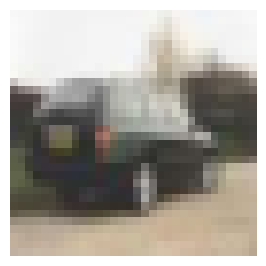
\includegraphics[width=\linewidth]{figures/cifar-images/automobile.png} \\
            \centering\scriptsize\texttt{automobile}
        \end{minipage} &
        \begin{minipage}[b]{0.15\linewidth}
            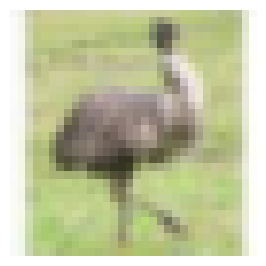
\includegraphics[width=\linewidth]{figures/cifar-images/bird.png} \\
            \centering\scriptsize\texttt{bird}
        \end{minipage} &
        \begin{minipage}[b]{0.15\linewidth}
            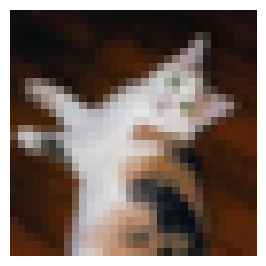
\includegraphics[width=\linewidth]{figures/cifar-images/cat.png} \\
            \centering\scriptsize\texttt{cat}
        \end{minipage} &
        \begin{minipage}[b]{0.15\linewidth}
            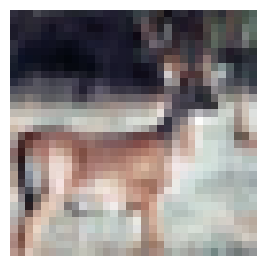
\includegraphics[width=\linewidth]{figures/cifar-images/deer.png} \\
            \centering\scriptsize\texttt{deer}
        \end{minipage} \\
        \begin{minipage}[b]{0.15\linewidth}
            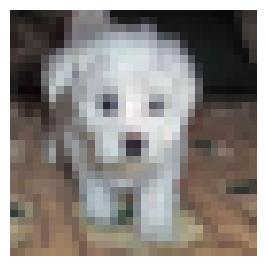
\includegraphics[width=\linewidth]{figures/cifar-images/dog.png} \\
            \centering\scriptsize\texttt{dog}
        \end{minipage} &
        \begin{minipage}[b]{0.15\linewidth}
            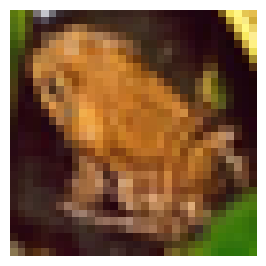
\includegraphics[width=\linewidth]{figures/cifar-images/frog.png} \\
            \centering\scriptsize\texttt{frog}
        \end{minipage} &
        \begin{minipage}[b]{0.15\linewidth}
            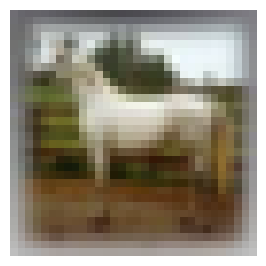
\includegraphics[width=\linewidth]{figures/cifar-images/horse.png} \\
            \centering\scriptsize\texttt{horse}
        \end{minipage} &
        \begin{minipage}[b]{0.15\linewidth}
            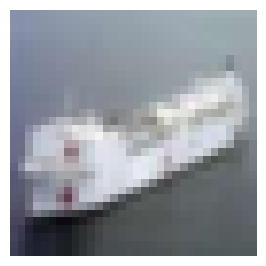
\includegraphics[width=\linewidth]{figures/cifar-images/ship.png} \\
            \centering\scriptsize\texttt{ship}
        \end{minipage} &
        \begin{minipage}[b]{0.15\linewidth}
            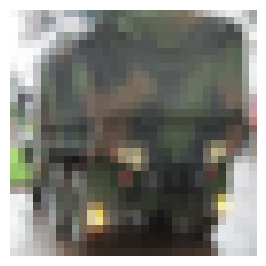
\includegraphics[width=\linewidth]{figures/cifar-images/truck.png} \\
            \centering\scriptsize\texttt{truck}
        \end{minipage}
    \end{tabular}
    \caption{Grid of example CIFAR-10 images. Classes are: airplane, automobile, bird, cat, deer, dog, frog, horse, ship, and truck (in order from left to right, top to bottom).}
    \label{fig:grid_images}
\end{figure}

\begin{figure}[ht]
    \centering
    \begin{subfigure}[b]{0.8\linewidth}
        \centering
        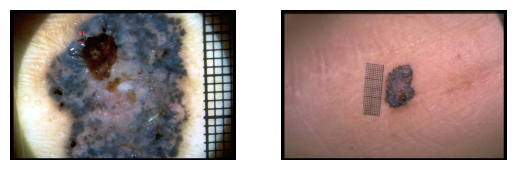
\includegraphics[width=\linewidth]{figures/derm7pt-images/derm_01.png}
        \vspace{0.25em}
        \raggedright
        \footnotesize\texttt{diagnosis}: basal cell carcinoma\\
        \footnotesize\texttt{pigment\_network}: absent\\
        \footnotesize\texttt{streaks}: absent\\
        \footnotesize\texttt{pigmentation}: absent\\
        \footnotesize\texttt{regression\_structures}: blue areas\\
        \footnotesize\texttt{dots\_and\_globules}: irregular\\
        \footnotesize\texttt{blue\_whitish\_veil}: present\\
        \footnotesize\texttt{vascular\_structures}: within regression\\
        \vspace{0.25em}
        \footnotesize\texttt{seven\_point\_score}: 4\\
        \footnotesize\texttt{level\_of\_diagnostic\_difficulty}: low
        \label{fig:first_image}
    \end{subfigure}
    
    \vspace{1em}
    
    \begin{subfigure}[b]{0.8\linewidth}
        \centering
        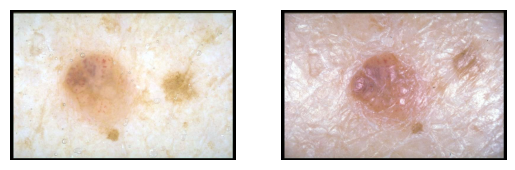
\includegraphics[width=\linewidth]{figures/derm7pt-images/derm_02.png}
        \vspace{0.25em}
        \raggedright
        \footnotesize\texttt{diagnosis}: melanoma metastasis\\
        \footnotesize\texttt{pigment\_network}: absent\\
        \footnotesize\texttt{streaks}: absent\\
        \footnotesize\texttt{pigmentation}: diffuse irregular\\
        \footnotesize\texttt{regression\_structures}: absent\\
        \footnotesize\texttt{dots\_and\_globules}: regular\\
        \footnotesize\texttt{blue\_whitish\_veil}: absent\\
        \footnotesize\texttt{vascular\_structures}: hairpin\\
        \vspace{0.25em}
        \footnotesize\texttt{seven\_point\_score}: 1\\
        \footnotesize\texttt{level\_of\_diagnostic\_difficulty}: high
        \label{fig:second_image}
    \end{subfigure}

    \caption{Example dermoscopic and clinical images from the Seven-Point Checklist Dermatology Dataset (Derm7Pt) with their corresponding diagnostic criteria and seven-point checklist scores.}
    \label{fig:derm_images}
\end{figure}

For our specialized medical imaging task, we employ the Seven-Point Checklist Dermatology Dataset (which we call Derm7Pt for brevity) dataset~\cite{Kawahara2019}, which consists of 1,011 dermatological cases. Each case includes both dermoscopic images (captured using a dermatoscope under standardized lighting and magnification) and clinical images (standard photographs taken at varying distances and lighting conditions and containing potential artifacts) along with patient metadata. The dataset is divided into training (413 cases), validation (203 cases), and test (395 cases) sets. The dataset is structured around two main types of labels: primary diagnosis (DIAG) (including categories such as melanoma, basal cell carcinoma, and various types of nevi) and the seven-point checklist criteria used in melanoma diagnosis. These seven criteria include pigment network (PN) characteristics, blue-whitish veil (BWV) presence, vascular structures (VS), pigmentation patterns (PIG), streaks (STR), dots/globules (DaG), and regression structures (RS), each with specific subcategories that aid in melanoma identification. Notably, Kawahara et al.~\cite{Kawahara2019} provide a library simplifying use of the dataset and groups infrequent labels with equivalent clinical interpretations into single general labels.

\subsection{Models Used}
We select models for their ability to process interleaved image and text inputs, and their claimed ability to handle multi-image, multi-turn multimodal conversations that align with the nature of the in-context few-shot learning method. Note that the parameter counts reported in this section are likely approximate, and are taken from the authors' Hugging Face model pages. We evaluate the following models in this work:

\begin{itemize}
    \item InternVL2-8B model~\cite{Chen2023}, which integrates \texttt{InternViT-300M-448px} for visual encoding with \texttt{InternLM2-5-7B-Chat} for language processing, totaling 8.08 billion parameters. This model has an 8k context window and can handle text, multiple images, and video inputs. The authors note however, that the limited availability of multi-image conversation data for training may lead to inconsistent performance on multi-image tasks.

    \item MiniCPM-V-2.6 model~\cite{Yao2024}, which integrates \texttt{SigLip-400M} for visual encoding, a perceiver resampler compression layer and \texttt{Qwen2-7B} for language processing, totaling 8 billion parameters. The visual tokens generated from preprocessed image slices are processed through the compression layer, which significantly reduces token count and \gls{gpu} memory usage while enhancing inference speed. Additionally, the authors note that the model employs a spatial schema to wrap and separate image tokens, facilitating improved spatial understanding. The model supports various input types, including single images, multiple images, and video content.
    
    \item Phi-3.5-vision-instruct model~\cite{Abdin2024}, which provides efficient multimodal processing with smaller model size. With 4.15 billion parameters, it includes a vision encoder for image understanding and supports a 128K context window for managing long sequences. This model is designed for memory and compute-constrained environments, and can perform multimodal tasks such as those involving single images, multi-image comparisons, and video clip summarization.

    \item Pixtral 12B~\cite{Agrawal2024}, which is a larger \gls{vl} model that combines a 400M parameter vision encoder trained from scratch with a 12B parameter multimodal decoder based on the Mistral Nemo model, totaling approximately 12.4 billion parameters. This model features a 128K context window and can handle variable image sizes and aspect ratios, processing images at their native resolution by converting them into image tokens for each 16x16 patch. The authors note that this design allows for the processing of both high-resolution documents and smaller images (such as icons or equations) while also keeping the ability to process multiple images within its context window.

    \item Bio-Medical-MultiModal-Llama-3-8B-V1~\cite{ContactDoctor2024}, which is a fine-tuned multimodal adaptation of Llama-3.1-8B-Instruct with 8.54 billion parameters. The authors claim that it has been trained on over 500,000 biomedical text and image entries. This model is included to examine whether this specialized training enhances the model's understanding of the concepts necessary for performing a specialized biomedical robotic vision task. Note that we only evaluate this model on the Seven Point Checklist Dermatology Dataset (Derm7Pt).
\end{itemize}

\subsection{Experimental Design}
Our experimental design comprises three main components to evaluate the following aspects:

\begin{enumerate}
    \item The models' ability to perform classification in a zero-shot learning/transfer context without the provision of prior examples is assessed. This evaluation is conducted through basic zero-shot prompting as well as enhanced prompts that include task-specific information and reasoning-based prompts that employ chain-of-thought techniques.
    
    \item Next, the models' ability to perform few-shot learning/transfer by assessing how the provision of examples influences model performance, as well as resource usage is explored. This exploration encompasses pure few-shot experiments with 1 to 16 examples, as well as combinations where examples are paired with zero-shot prompting, and where examples are combined with enhanced task information in the prompt.
    
    \item Finally, our experimental design includes a focus on downstream model training, where we evaluate knowledge transfer by utilizing VLM-generated pseudolabels to train lightweight models. In this phase, we compare the performance of these models against those trained on ground truth labels and analyze the effects of various transfer methods on downstream performance.
\end{enumerate}

\subsection{Metrics and Resource Analysis}
To ensure a comprehensive evaluation, we employ analogous metrics for both datasets. For CIFAR-10, we consider basic accuracy over the classes of the dataset. In the case of the Derm7Pt dataset, we compute the accuracy over each of the seven categories to compute tag-specific and overall average accuracy, as well as introduce a random-guessing accuracy baseline to assist in the analysis of the performance of the models.

To analyze performance and resource scaling, a computational resource analysis is conducted, tracking and analyzing memory usage and time usage patterns across different shot counts and experiment configurations.

\subsection{Prompting and VLM Input}
The prompting strategy aims to systematically evaluate vision-language models' capabilities in both general and specialized classification tasks while maintaining reproducibility and fairness in comparisons. The core objectives of the prompting framework are:
\begin{itemize}
    \item To establish a consistent interaction format that enables fair comparison across different models and tasks
    \item To isolate the effects of different prompting components (zero-shot instructions, few-shot examples, reasoning requirements) on model performance for analysis
    \item To minimize potential biases due to the ordering of examples through systematic randomization of class lists and example ordering
    \item To maintain reproducibility through deterministic and balanced random example selection and standardized prompt templates
\end{itemize}

The framework implements a chat-based interaction format that maintains consistency across all experiments while accommodating task-specific requirements. The core structure consists of three main components:

    \begin{enumerate}
    \item \emph{Base Prompt Structure:} Each interaction begins with a task definition, including a randomized class list to mitigate position bias, and a response format specification. For few-shot scenarios, this initial prompt (if used) appears only once at the start of the conversation to avoid redundancy.

    \item \emph{Example Integration:} In few-shot scenarios, examples are presented through alternating user-assistant message pairs. Each user message contains a numbered image reference (e.g., "Image-1"), while each assistant message contains only the corresponding label or classification. This maintains a clean separation between examples and ensures consistent formatting across all models. Note that the assistant messages here are provided by the user, and not generated by the model.

    \item \emph{Test Instance Presentation:} The final turn in each conversation presents the test image as a user message using the same numbering scheme as the examples. This standardization ensures that models can reliably identify the image requiring classification, regardless of the surrounding context.
    \end{enumerate}

To ensure reproducibility and fairness, the framework implements several key controls:
\begin{itemize}
    \item Deterministic random seeds for both class list shuffling and example selection -- each model is provided exactly the same input, inclusive of the class-list and example ordering, for each example from the dataset. The random seeds are incremented for each example from the dataset.
    \item Balanced representation of classes in few-shot examples -- for each example, the possible classes are represented equally in the examples included.
    \item Explicit exclusion of test images from the example selection pool -- the test example at the end is not included as an example sampled from the dataset.
    \item Standardized image preprocessing over the entire dataset when required.
\end{itemize}

This core framework is then adapted for two distinct classification scenarios:

\paragraph{CIFAR-10 Classification Implementation}
For the CIFAR-10 dataset, we implement a straightforward adaptation of the core framework focused on single-label classification. The base prompt establishes the classification task and provides a randomized list of the ten possible classes. To investigate different prompting strategies, we developed variants of increasing complexity: basic 0-shot with minimal instructions, 0.5-shot with class-specific context (e.g., distinguishing trucks from automobiles), and reasoning-based prompts requiring step-by-step observation and justification before classification. An example of how the prompt is built for the CIFAR-10 dataset is shown in \autoref{fig:prompt-building}.

For few-shot scenarios, examples are integrated following the core framework's turn-based structure, with each example consisting of a single image and its corresponding label. The class order of the examples is randomized for each conversation to mitigate potential position bias in the model's predictions.

\paragraph{Derm7Pt Medical Analysis Implementation}
The Derm7Pt implementation extends the framework to handle both structured feature analysis and direct diagnosis tasks. This adaptation manages increased complexity in three key aspects: multiple classification tasks per image, optional inclusion of clinical images alongside dermoscopic images, and specialized medical information context requirements.

For feature analysis, we structure the prompt to address each of the seven checklist criteria separately, maintaining clear task guidelines for each category. The diagnostic task uses a comprehensive class list while incorporating relevant medical context. Both tasks support the optional inclusion of clinical images as additional context. Additional task information can also be optionally provided in the structured feature analysis task. In few-shot scenarios, examples maintain the turn-based structure but may include multiple images (dermoscopic and clinical) per turn. 

For both scenarios, the models' textual responses are normalized before validation against valid entries in the class list and evaluating correctness. When reasoning is enabled, the models are prompted to generate detailed descriptions of image features and reason about the image before classification. Since reasoning requirements often result in long responses, the models were prompted to generate the final classification in a certain format (within angle brackets). In case the model failed to generate a response in the expected format, the response would also be processed using fallback formats that were noted in such examples (quotation marks, for example).

\begin{figure}[ht]
    \centering
    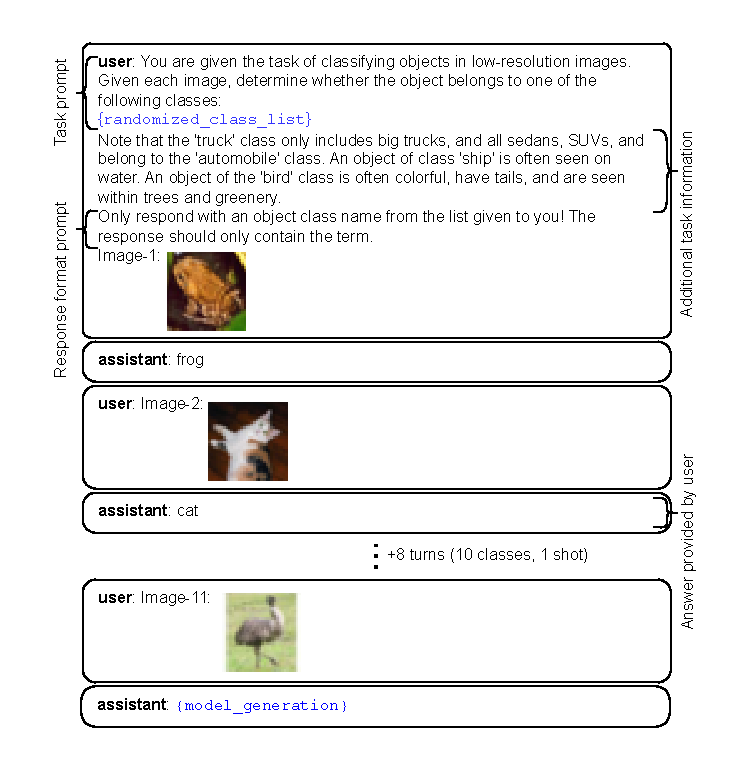
\includegraphics[width=\linewidth]{figures/prompt_building.pdf}
    \caption{Visualization of the prompt building process for the CIFAR-10 dataset. A similar process is used for the Derm7Pt dataset, but with category-specific prompts for each category and the optional addition of clinical images. See Appendix~\ref{sec:appendix:prompts} for the complete prompt structures.}
    \label{fig:prompt-building}
\end{figure}

Over the course of the zero-shot experiments, it was noted that the Pixtral 12B model would initially always claim in the generated output that it could not see the image provided to it. To mitigate this issue, images were resized to 224x224 pixels before being provided to the Pixtral 12B model, which resolved the issue. We hypothesize that this is due to the model processing images at their native resolution, which means that the 32x32 images from the CIFAR-10 dataset were being encoded into approximately four tokens and too little information was being provided to the model to be able to make a prediction. Notably, all other models perform their own tiling and resizing of the images, which means that image processing techniques vary between models. For the Derm7Pt dataset, we encountered memory limitations when attempting to utilize more than two shots in our few-shot experiments due to the high resolution of the images. To address this, we resized all images to 224x224 pixels before providing them to the models, enabling the provision of more shots/examples.

\subsection{Downstream Models and Training}
Our downstream experiments investigate the effectiveness of using VLM-generated pseudolabels for training smaller, task-specific models. We focus primarily on the CIFAR-10 dataset (due to unsatisfactory performance of the models on the Derm7Pt dataset), evaluating our approach using both the original ground truth labels as baseline and pseudolabels generated by four different VLMs: Pixtral-12B, InternVL-2, MiniCPM-V2.6, and Phi-3.5 Vision Instruct. This diverse set of models allows us to assess the robustness and generalizability few-shot VLM transfer across different model architectures, sizes, and capabilities.

For the downstream architecture, we employ a ResNet-18 model~\cite{He2016} pre-trained on ImageNet~\cite{Deng2009}. While ImageNet pre-training and fine-tuning has been a conventional paradigm in computer vision, He et al.~\cite{He2019} demonstrated that models trained from random initialization can achieve comparable performance. Their findings suggest that pre-training primarily accelerates early convergence rather than providing regularization benefits or improving final task accuracy. Nevertheless, we utilize the pre-trained model as our starting point, modifying its output layer to accommodate the 10-class classification task.

Our training methodology encompasses three main components. First, we employ full fine-tuning of the entire network using an \texttt{AdamW} optimizer with a learning rate of \(1 \times 10^{-5}\), allowing all parameters to adapt to the target task. Second, we experiment with two loss function variants: a standard cross-entropy loss and a label smoothing cross-entropy loss (smoothing=0.5) for potentially improved regularization. We hypothesize that label smoothing could be beneficial when training with potentially noisy pseudolabels. Finally, we explore two distinct VLM-generated data utilization approaches: direct use of pseudolabels for training, and an ablation study where we train on ground-truth labels only for examples where pseudolabels are valid, allowing us to analyze the specific impact of pseudolabel noise on downstream model performance.

Our experimental framework systematically evaluates this approach across multiple dimensions, assessing performance with different VLM architectures and training configurations while maintaining careful comparison against ground truth baselines. Through this comprehensive evaluation, we analyze the effectiveness of VLMs in generating pseudolabels, their comparative performance against ground truth training, and the optimal approaches for leveraging VLMs in generating pseudolabels for practical image classification tasks.
   
\end{document}
